% !TEX encoding = UTF-8 Unicode
\documentclass{article}

\usepackage{polski}
\usepackage[utf8]{inputenc}
\usepackage{subfig}
\usepackage{multirow}
\usepackage{graphicx}

\usepackage[a4paper, left=2.5cm, right=2.5cm, top=3.5cm, bottom=3.5cm, headsep=1.2cm]{geometry}

\linespread{1.3}
\begin{document}
	
	\begin{titlepage}
		\centering
		{\scshape\LARGE Politechnika Wrocławska \par}
		{\scshape\Large Katedra Informatyki Technicznej\par}
		
		\vspace{1cm}
		{\scshape\Large Inżynieria Oprogramowania\par}
		\vspace{1.5cm}
		{\huge\bfseries \par}
		\vspace{2cm}
		{\Large\itshape Magdalena Biernat\par}
		{\Large\itshape Mateusz Bortkiewicz\par}
		\vfill
		Opiekun\par
		prof. dr hab. inż. Jan Magott 
		
		\vfill
		{\large \today\par}
	\end{titlepage}
	\newpage
	
	\section{Wprowadzenie}
	Sprawozdanie dotyczy dziewiątych i dziesiątych zajęć. Na tych laboratoriach kontynuowaliśmy swój projekt. 
	
	\subsection{Cel laboratorium}
	Definiowanie w sposób iteracyjno - rozwojowy modelu projektowego
	programowania opartego na:
	\begin{itemize}
		\item Modelowaniu logiki biznesowej reprezentowanej przez wybrany
		przypadek użycia za pomocą diagramów sekwencji po wykonaniu
		pierwszego przypadku użycia podczas laboratorium 8, stanowiącego
		bazową logikę biznesową, z której korzystają kolejne przypadki użycia.
		Należy definiować operacje i atrybuty kolejnej klasy (dziedziczenie,
		powiązania i agregacje) na diagramie klas zidentyfikowanej w wyniku
		modelowania kolejnego przypadku użycia i wykonanie scenariusza tego
		przypadku użycia za pomocą diagramu sekwencji.
		\item Implementacja modelu projektowego wybranego przypadku użycia za
		pomocą języka Java SE – rozszerzanie kodu źródłowego programu
		wykonanego podczas laboratoriów 7 i 8.
	\end{itemize}
	\subsection{Plan pracy}
	Zadania wykonaliśmy wg instrukcji 7:
	\begin{itemize}
		\item Wykonanie diagramów sekwencji.
		\item Poprawa diagramu klas.
		\item Implementacja kodu w javie.
	\end{itemize}
\newpage
\section{Laboratorium}
\subsection{Wykonane diagramy sekwencji}
\subsubsection{Diagram sekwencji zwrotu}
\begin{figure}[!ht]
	\centering
	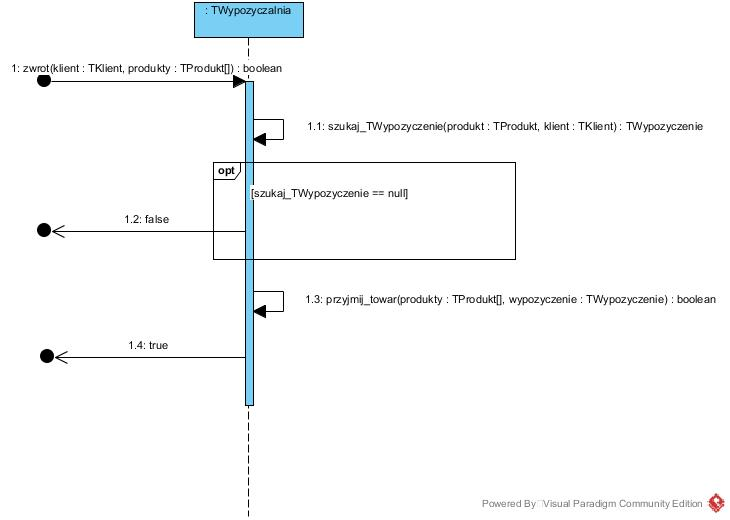
\includegraphics[angle=270,width=13cm]{5.jpg}
	\caption{Stworzony diagram sekwencji}
	\label{fig:obrazek 1}
	\newpage
\end{figure}
\subsubsection{Diagram sekwencji wypożyczenia}
\begin{figure}[!ht]
	\centering
	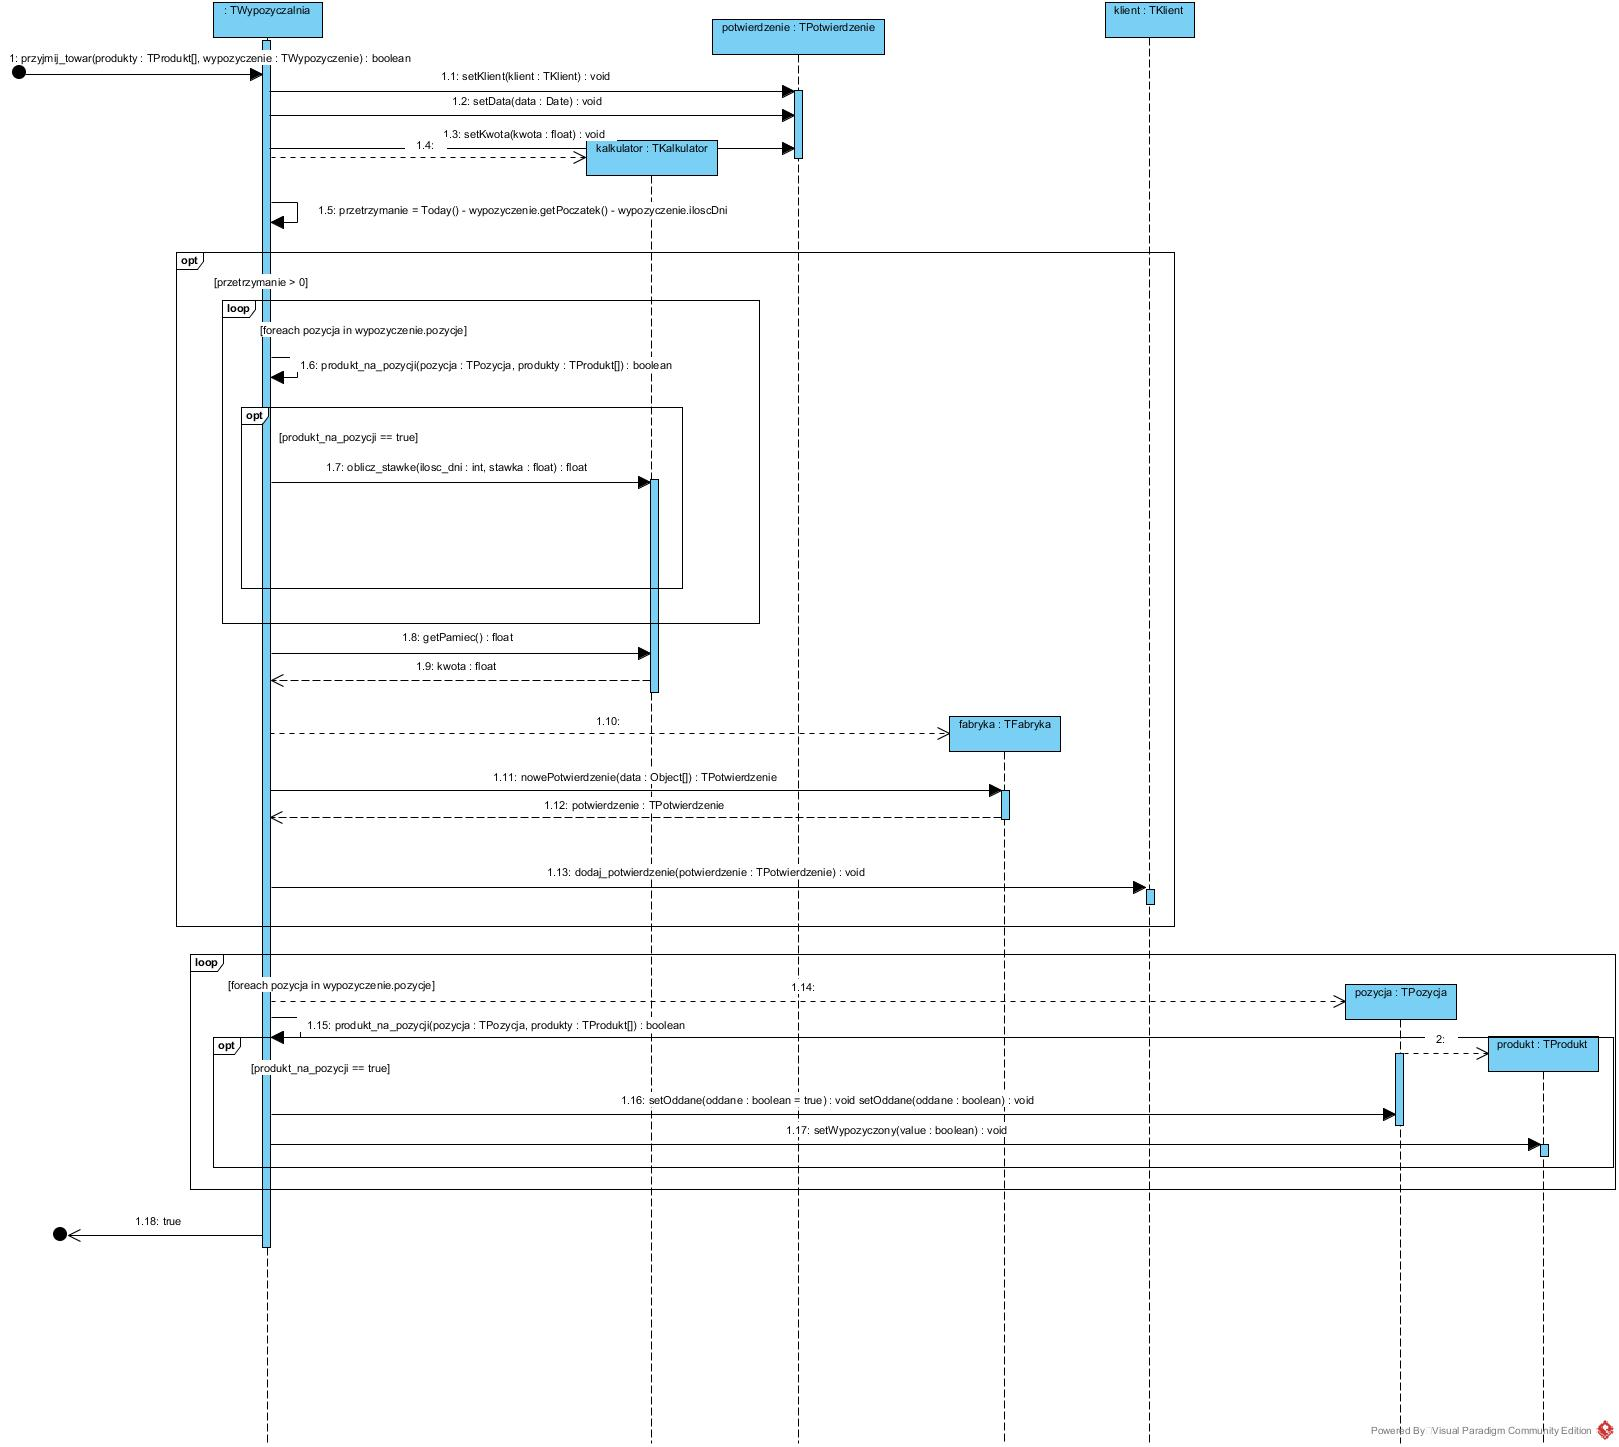
\includegraphics[angle=270,width=17cm]{2.jpg}
	\caption{Stworzony diagram sekwencji}
	\label{fig:obrazek 2}
\end{figure}
\newpage
\subsubsection{Diagram sekwencji Szukanie wypożyczenia}
\begin{figure}[!ht]
	\centering
	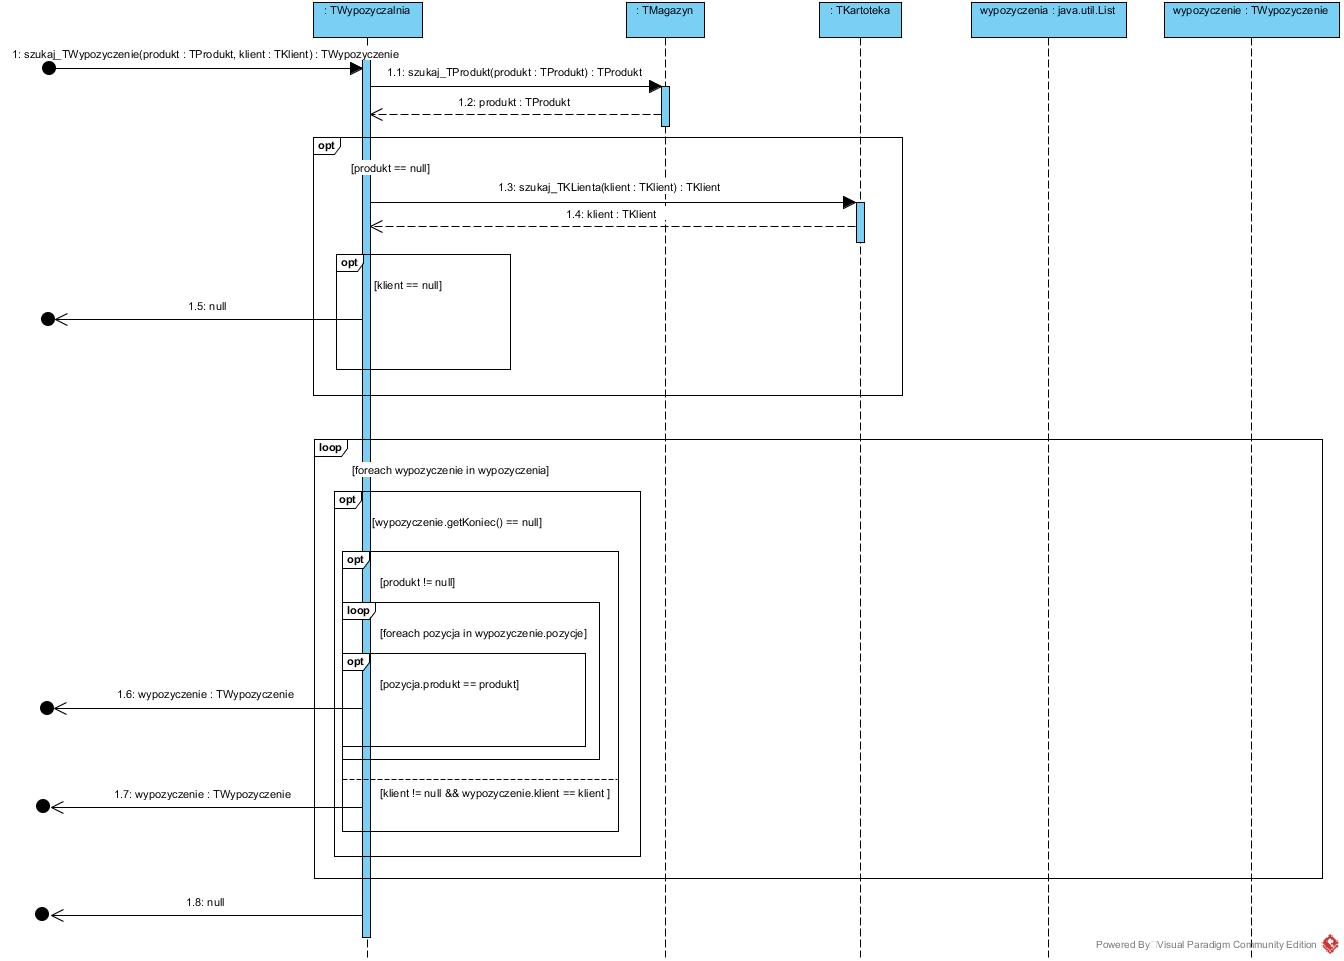
\includegraphics[angle=270,width=14cm]{3.jpg}
	\caption{Stworzony diagram sekwencji}
	\label{fig:obrazek 3}
\end{figure}
\newpage
\subsubsection{Diagram sekwencji PU Obliczanie terminu zwrotu i kosztu wypożyczenia}
\begin{figure}[!ht]
	\centering
	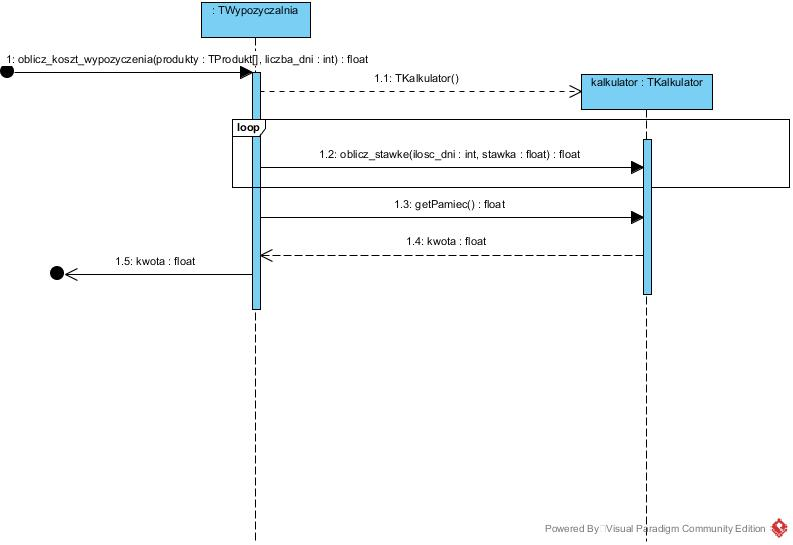
\includegraphics[angle=270,width=14cm]{1.jpg}
	\caption{Stworzony diagram sekwencji}
	\label{fig:obrazek 4}
\end{figure}
\subsubsection{Diagram sekwencji PU Przyjęcie towaru}
\begin{figure}[!ht]
	\centering
	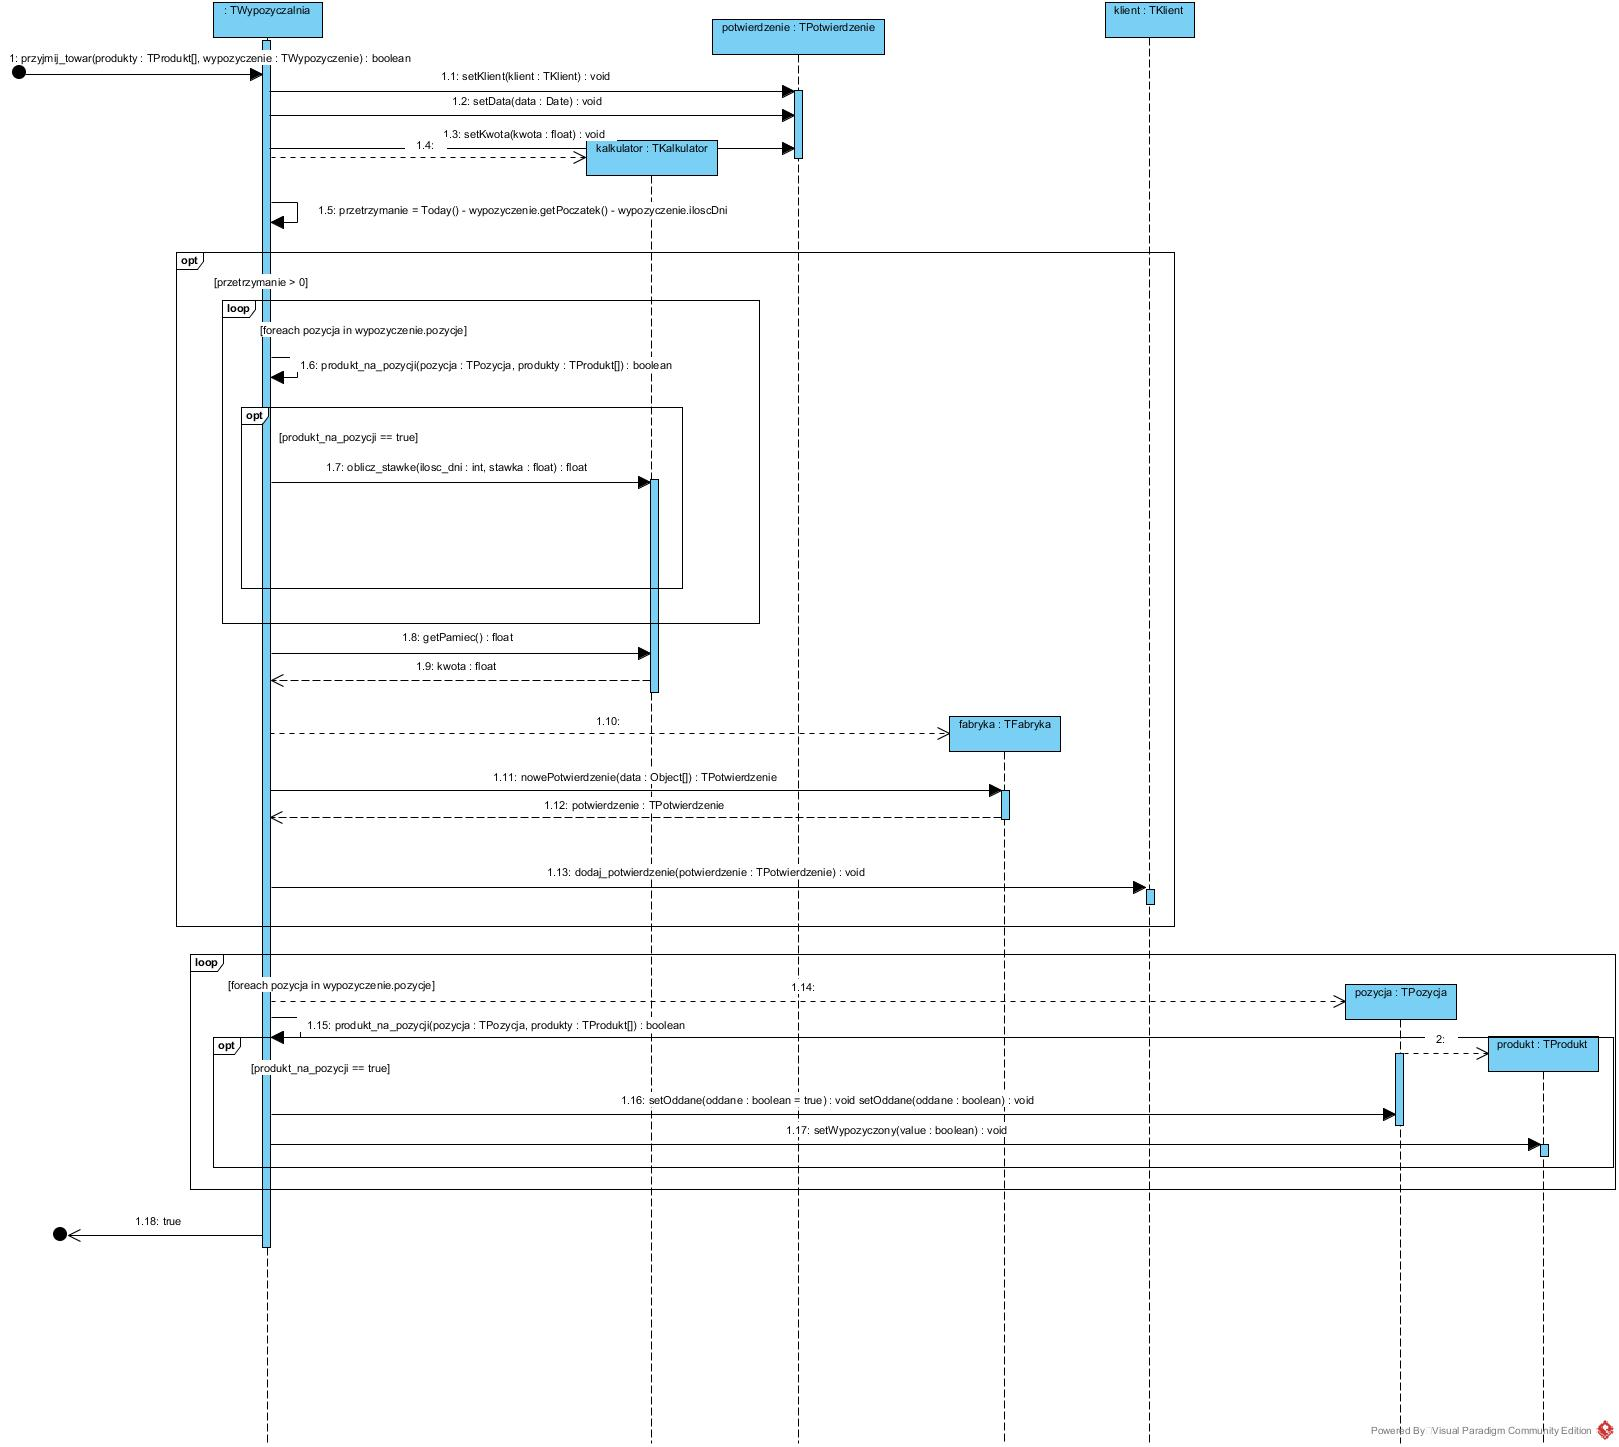
\includegraphics[angle=270,width=18cm]{2.jpg}
	\caption{Stworzony diagram sekwencji}
	\label{fig:obrazek 5}
\end{figure}
\subsection{Diagram klas}
\begin{figure}[!ht]
	\centering
	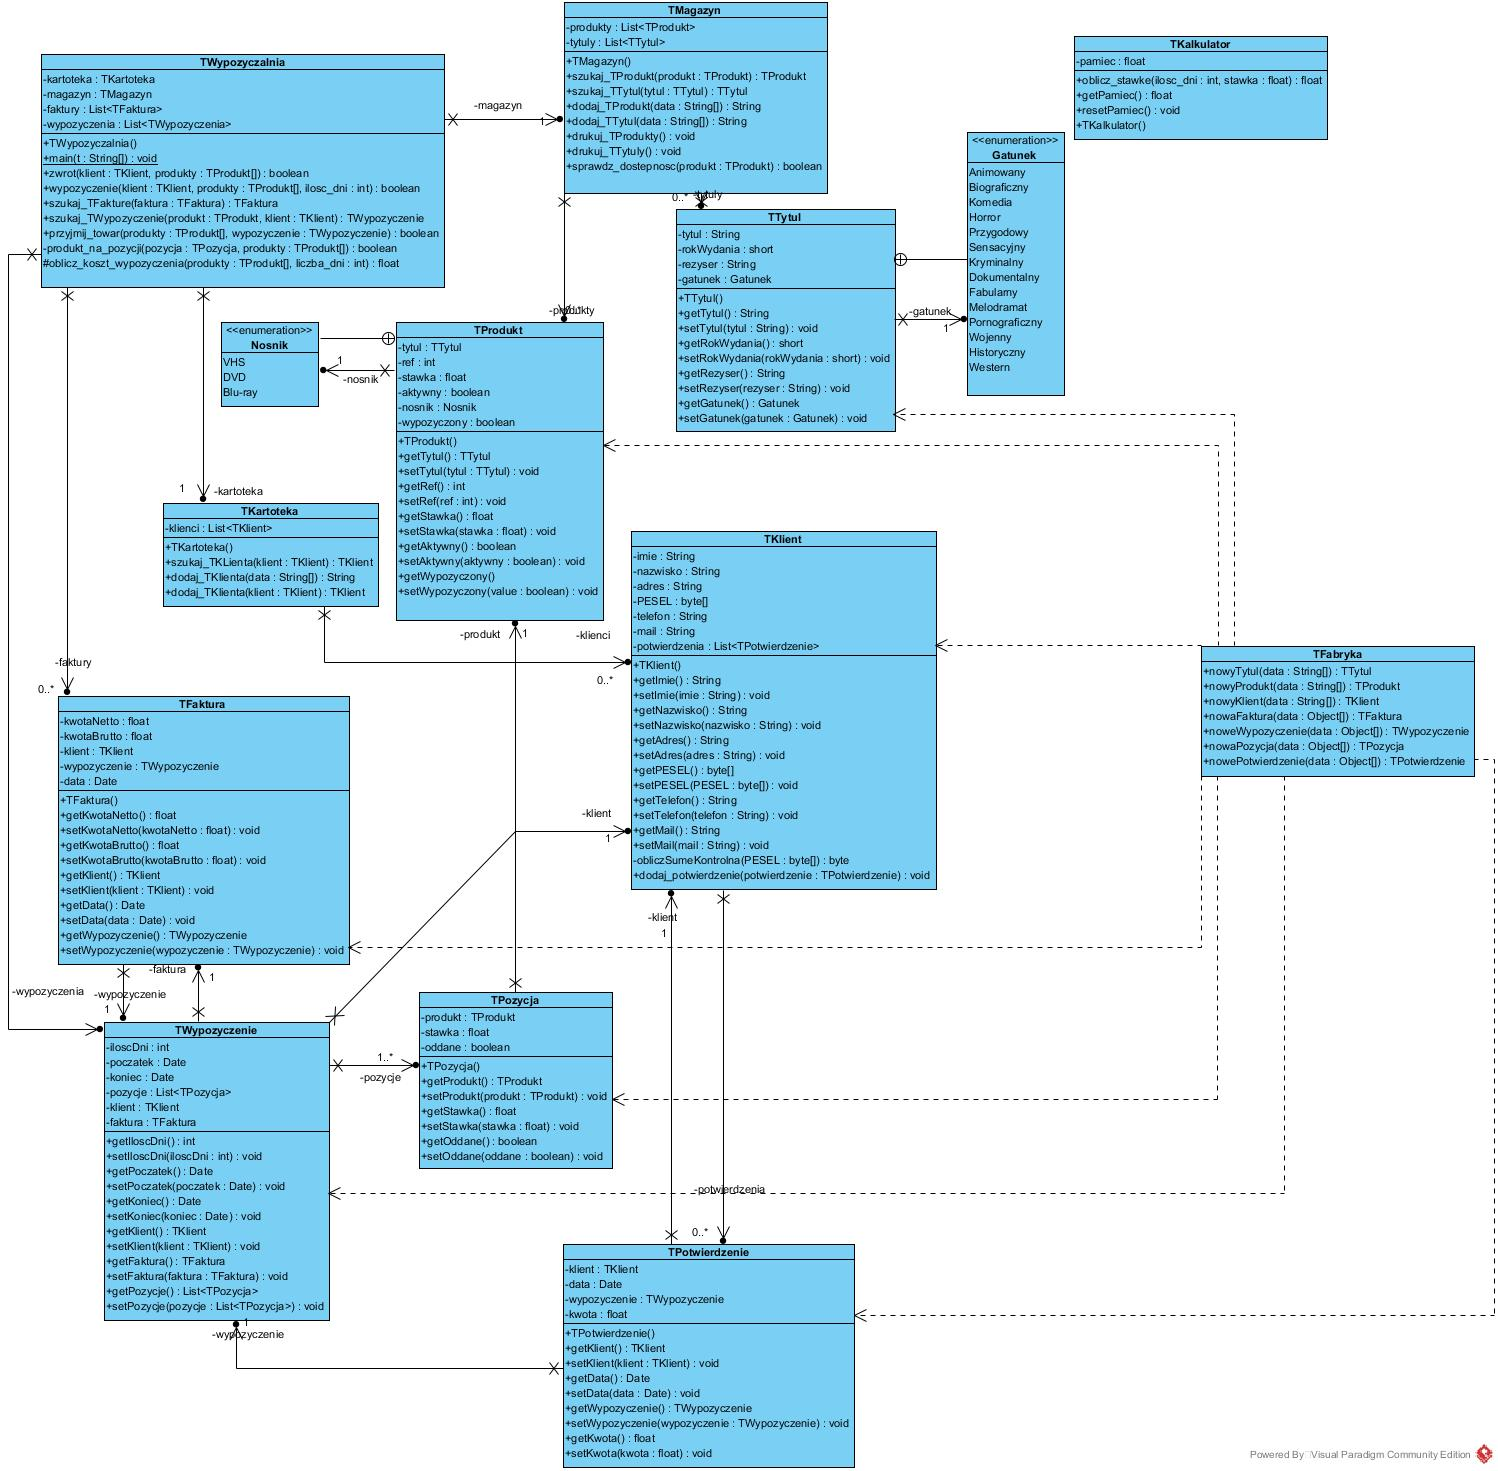
\includegraphics[width=17cm]{6.jpg}
	\caption{Poprawiony diagram klas
	}
	\label{fig:obrazek 6}
\end{figure}
\newpage
\subsection{Kod w javie}
Poniżej zawartość klasy TWypozyczalnia.
\begin{verbatim}
import java.util.ArrayList;
import java.util.Calendar;
import java.util.List;
import java.util.Date;

public class TWypozyczalnia {
	
	private TKartoteka kartoteka;
	private TMagazyn magazyn;
	private List<TFaktura> faktury;
	private List<TWypozyczenie> wypozyczenia;
	
	public TWypozyczalnia()	{
		super();
	}
	
	public static void main(String[] t)	{
		return;
	}
	
	public boolean zwrot(TKlient klient, TProdukt[] produkty)	{
		TWypozyczenie wypozyczenie = szukaj_TWypozyczenie(produkty[0], klient);
		
		if(wypozyczenie == null)
		return false;
		else {
			przyjmij_towar(produkty, wypozyczenie);
			return true;
		}
	}
	
	public boolean wypozyczenie(TKlient klient, TProdukt[] produkty, int ilosc_dni)	{
		TKlient nowyKlient;
		TKalkulator kalkulator = new TKalkulator(); 
		TFabryka fabryka = new TFabryka();
		TWypozyczenie wypozyczenie;
		TFaktura faktura;
		
		boolean dostepnosc;
		float kwota;
		
		for(int i=0; i < produkty.length; i++)		{
			dostepnosc = magazyn.sprawdz_dostepnosc(produkty[i]);
			
		if(dostepnosc == false) 
			return false;
		}
		
		nowyKlient = kartoteka.szukaj_TKlienta(klient);    
		
		if(nowyKlient == null)
			nowyKlient = kartoteka.dodaj_TKlienta(klient);
		
		for(int i =0; i < produkty.length; i++)
			kalkulator.oblicz_stawke(ilosc_dni, produkty[i].getStawka());
		
		kwota = kalkulator.getPamiec();
		List<TPozycja> pozycje = new ArrayList<TPozycja>();
		for(int i=0; i < produkty.length; i++)
			pozycje.add(fabryka.nowaPozycja(new Object[]{produkty[0], produkty[0].getStawka(), false}));
				
		wypozyczenie = fabryka.noweWypozyczenie(new Object[]{ilosc_dni, Calendar.getInstance().getTime(), null, pozycje, nowyKlient, null});
		faktura = fabryka.nowaFaktura(new Object[]{100*kwota/123, kwota, nowyKlient, wypozyczenie, wypozyczenie.getPoczatek()});
		wypozyczenie.setFaktura(faktura);
		faktury.add(faktura);
		wypozyczenia.add(wypozyczenie);
		
		return true;
	}
	
	public TFaktura szukaj_TFakture(TFaktura faktura) {
		return null;
	}
	
	public TWypozyczenie szukaj_TWypozyczenie(TProdukt produkt, TKlient klient)	{
		produkt = magazyn.szukaj_TProdukt(produkt);
		
		if(produkt==null) {
			klient = kartoteka.szukaj_TKlienta(klient);
			if(klient==null) 
				return null;
		}
		
		for(TWypozyczenie wypozyczenie : wypozyczenia)	{
			if(wypozyczenie.getKoniec()==null) 
			{
				if(produkt != null)	{
					for(TPozycja pozycja : wypozyczenie.getPozycje())	{
						if(pozycja.getProdukt() == produkt)
						return wypozyczenie;
					}          
				}
				else if(klient != null && wypozyczenie.getKlient() == klient)
					return wypozyczenie;
			}
		}
		return null;
	}
	
	public boolean przyjmij_towar(TProdukt[] produkty, TWypozyczenie wypozyczenie) {
		TKalkulator kalkulator = new TKalkulator();
		int przetrzymanie = daysBetween(Calendar.getInstance().getTimeInMillis(), wypozyczenie.getPoczatek().getTime()) - 
		wypozyczenie.getIloscDni();
		float kwota;
		if (przetrzymanie > 0) {
			for(TPozycja pozycja : wypozyczenie.getPozycje()) {
				if(produkt_na_pozycji(pozycja, produkty)) {
					kwota = kalkulator.oblicz_stawke(przetrzymanie, pozycja.getStawka());
				}
				
				kwota = kalkulator.getPamiec();
				TFabryka fabryka = new TFabryka();
				TPotwierdzenie potwierdzenie = fabryka.nowePotwierdzenie(new Object[]{Calendar.getInstance().getTimeInMillis(), 
					wypozyczenie.getKlient(), 
					kwota, 
					wypozyczenie});
				wypozyczenie.getKlient().dodaj_potwierdzenie(potwierdzenie);
			}
			
			for(TPozycja pozycja : wypozyczenie.getPozycje()) {
				boolean produkt = produkt_na_pozycji(pozycja, produkty);
				if(produkt) {
					pozycja.setOddane(true);
					pozycja.getProdukt().setWypozyczony(false);
				}
			}    
		}
		
		return true;
	}
	
	private boolean produkt_na_pozycji(TPozycja pozycja, TProdukt[] Produkty) {
		return false;
	}
	
	private int daysBetween(long t1, long t2) {
		return (int) ((t2 - t1) / (1000 * 60 * 60 * 24));
	} 
}
\end{verbatim}

\end{document}